\documentclass{theozettel}

%%%%%%%%%%%%%%%%%%%%%%%%%%%%%%%%%%%%%%%%%%%%%%%%%%%%%%%%%%%%%%%%%%%%%%%%%%%%%%%%%%%%%%%%%%%%%%%%%%%%%%%%%%%%%%
% page geometry
%%%%%%%%%%%%%%%%%%%%%%%%%%%%%%%%%%%%%%%%%%%%%%%%%%%%%%%%%%%%%%%%%%%%%%%%%%%%%%%%%%%%%%%%%%%%%%%%%%%%%%%%%%%%%%
\geometry{
	left=20mm,
	right=20mm,
	top=25mm,
	bottom=20mm
}
%%%%%%%%%%%%%%%%%%%%%%%%%%%%%%%%%%%%%%%%%%%%%%%%%%%%%%%%%%%%%%%%%%%%%%%%%%%%%%%%%%%%%%%%%%%%%%%%%%%%%%%%%%%%%%

\pgfplotsset{compat=1.16}

%\renewcommand{\phi}{\varphi}

\usepackage{parskip}
\usepackage{dsfont}
\newcommand{\difd}{\text{d}}
\usepackage{titlesec} 
\titleformat{\section}[runin]
{\normalfont\large\bfseries}{\thesubsection}{1em}{}
\titleformat{\subsection}[runin]
  {\normalfont\normalsize\bfseries}{\thesubsubsection}{1em}{}
  
\renewcommand{\epsilon}{\varepsilon}
\newcommand{\vol}{\operatorname{vol}}

\theoI{10}

\begin{document}
\punkteV{10.1}{10.2}{10.3}{10.4}{10.5}

\section*{Aufgabe 10.1}

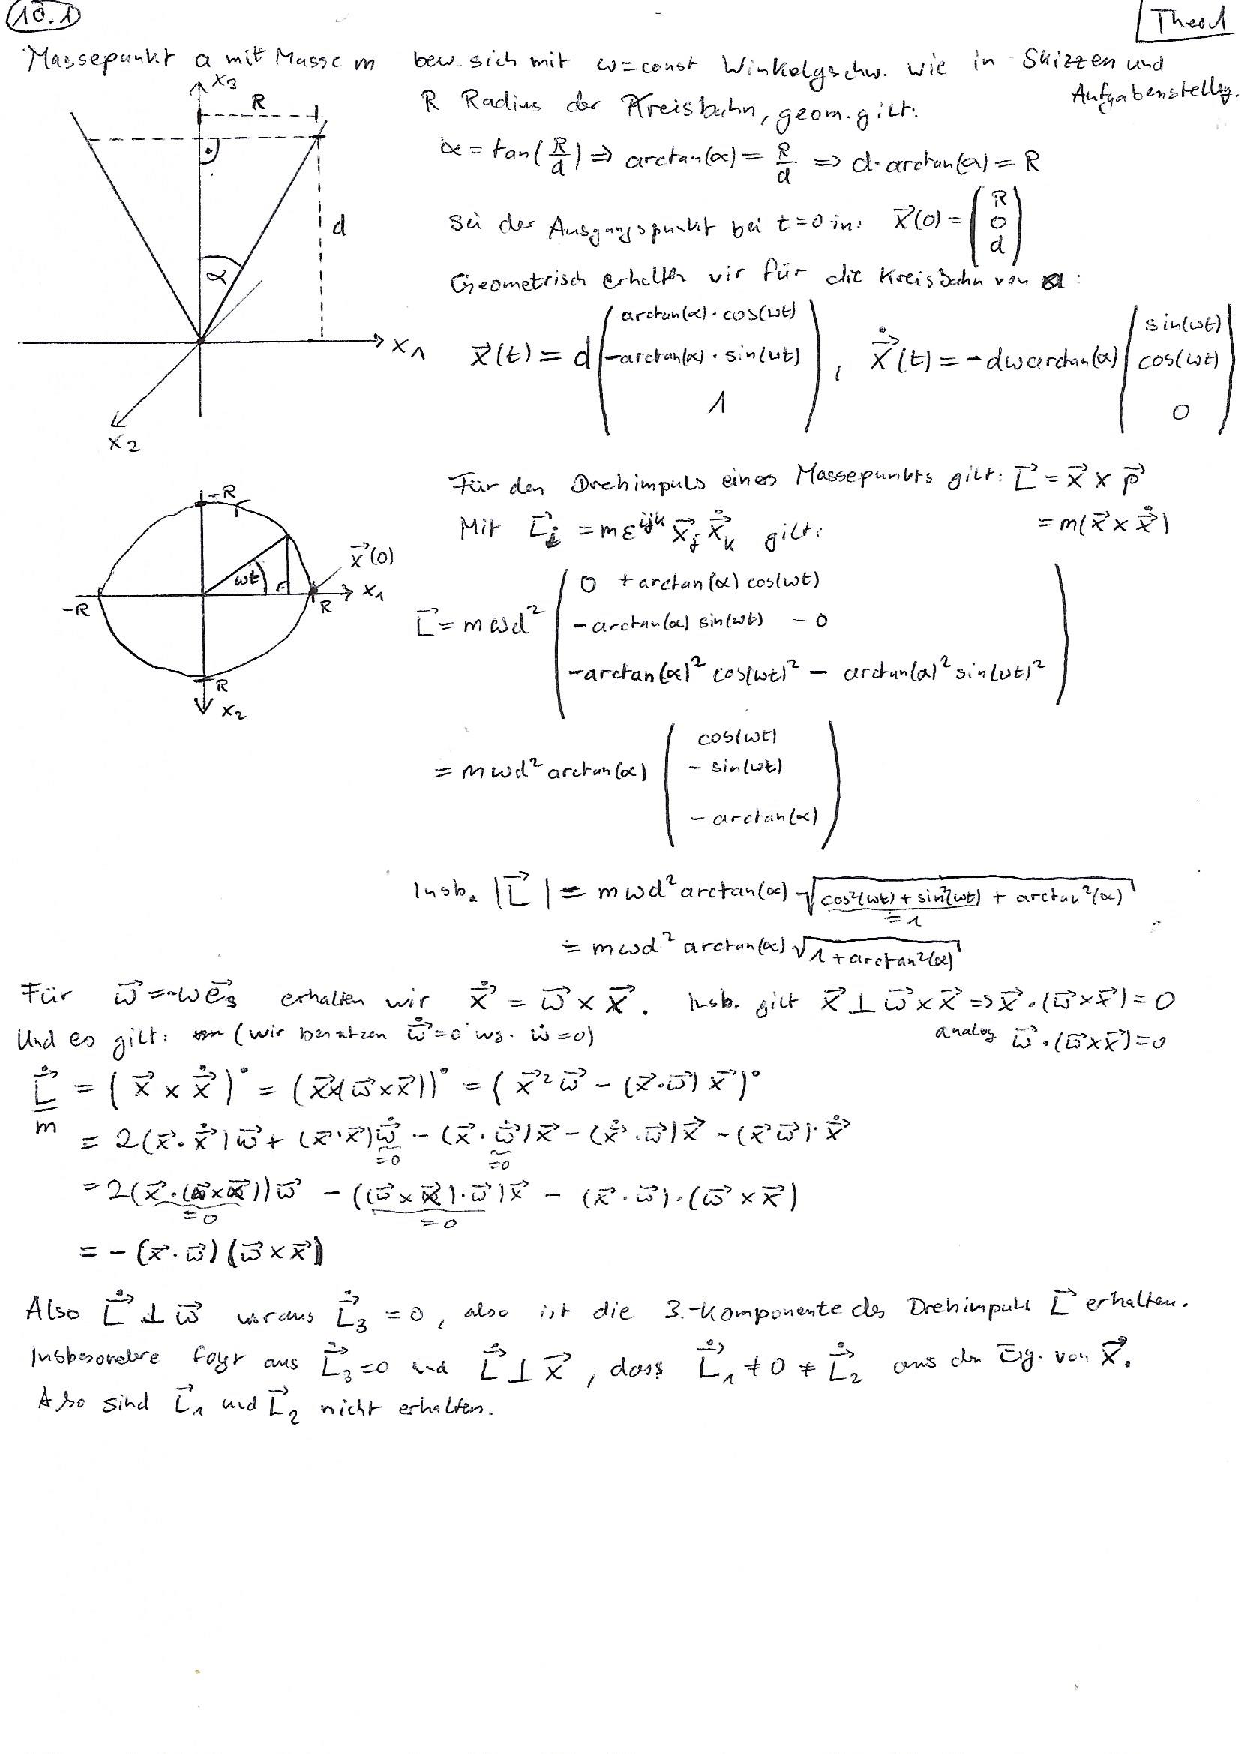
\includepdf[pages=-]{Theo1U10A1.pdf}



\section*{Aufgabe 10.2} 

Bei Aufgabe a) ist $s = l$ die Seitenlänge des Quadrats. Ich habe gedacht das Quadrat selbst hätte eine homogene Massenverteilung, und nicht, dass nur Punktmassen an den Ecken sind, was mir erst am Ende aufgefallen ist. Ich hatte leider keine Zeit mehr die Lösung zu ändern.

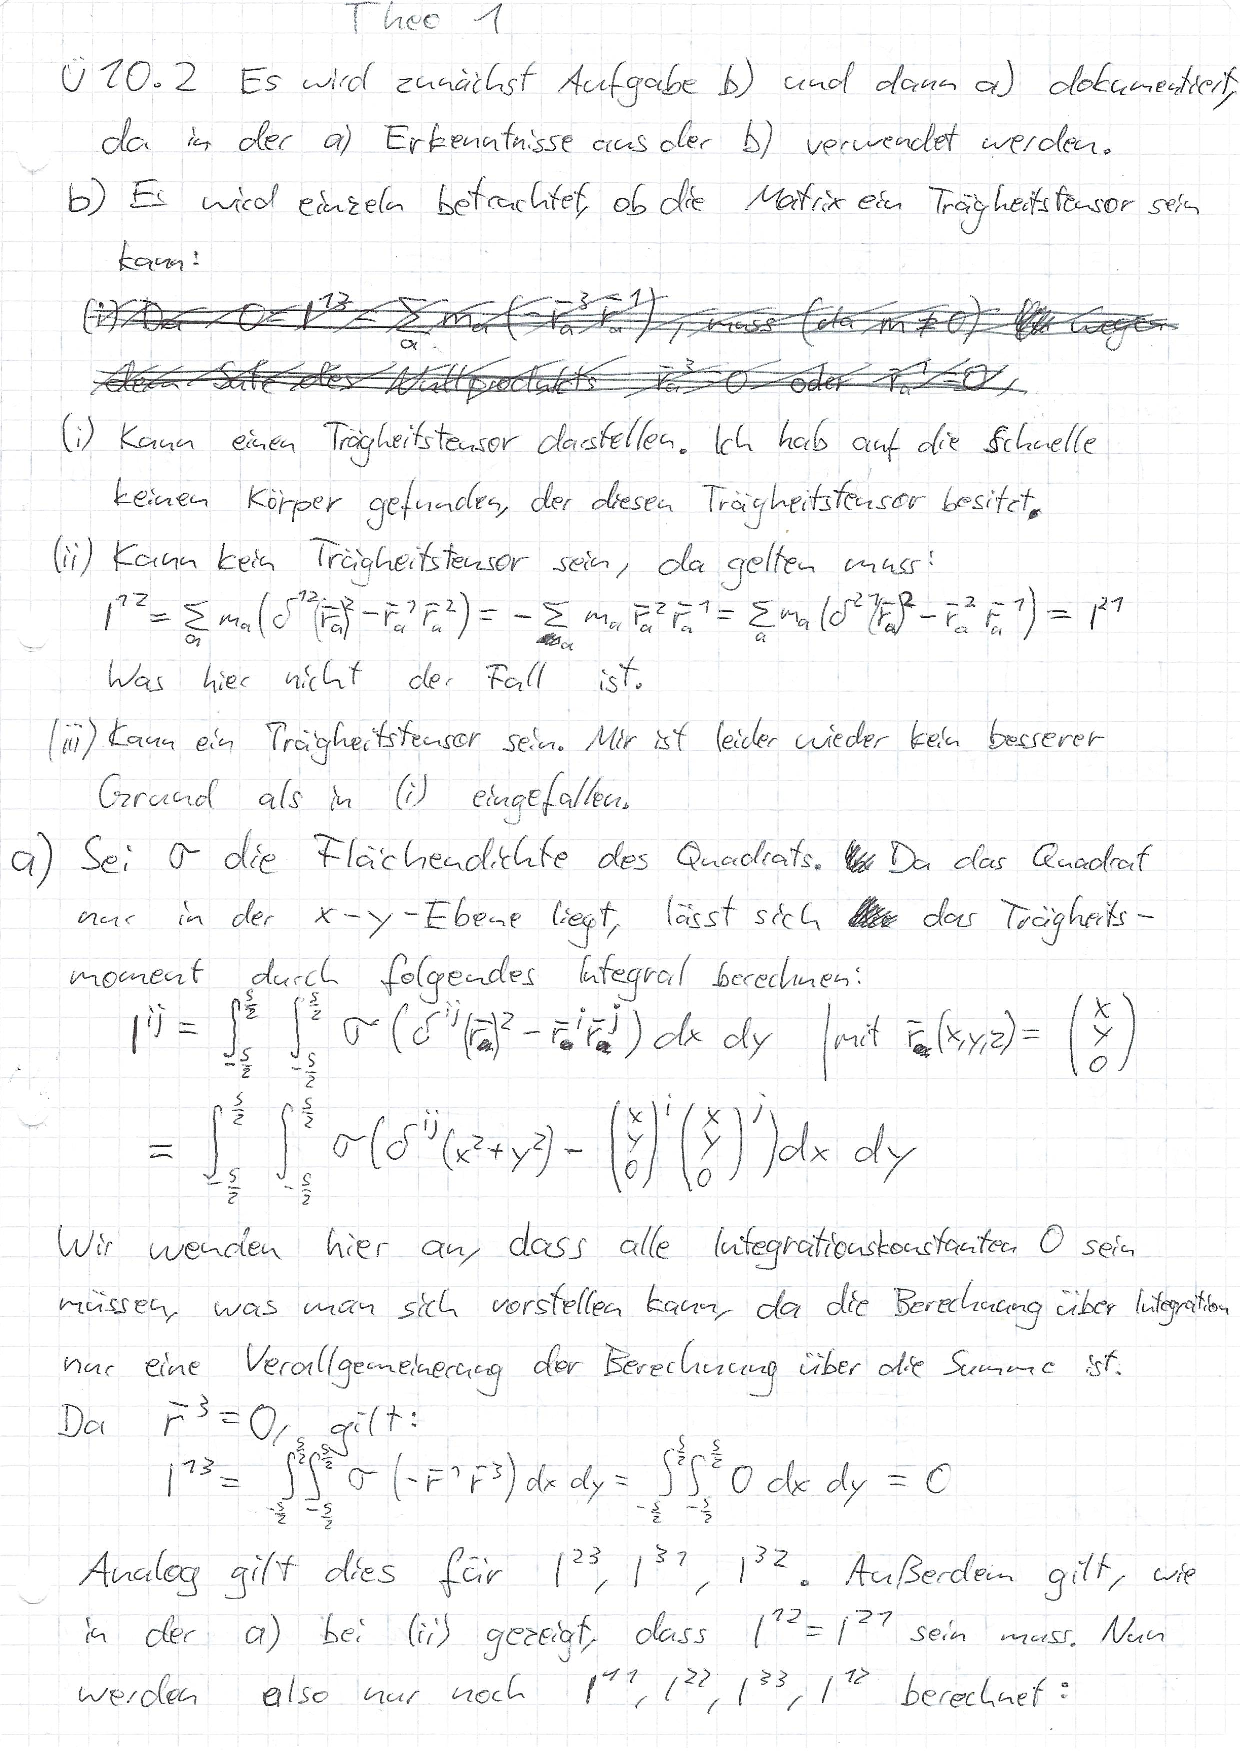
\includepdf[pages=-]{Theo1U10A2.pdf}

\section*{Aufgabe 10.3} 
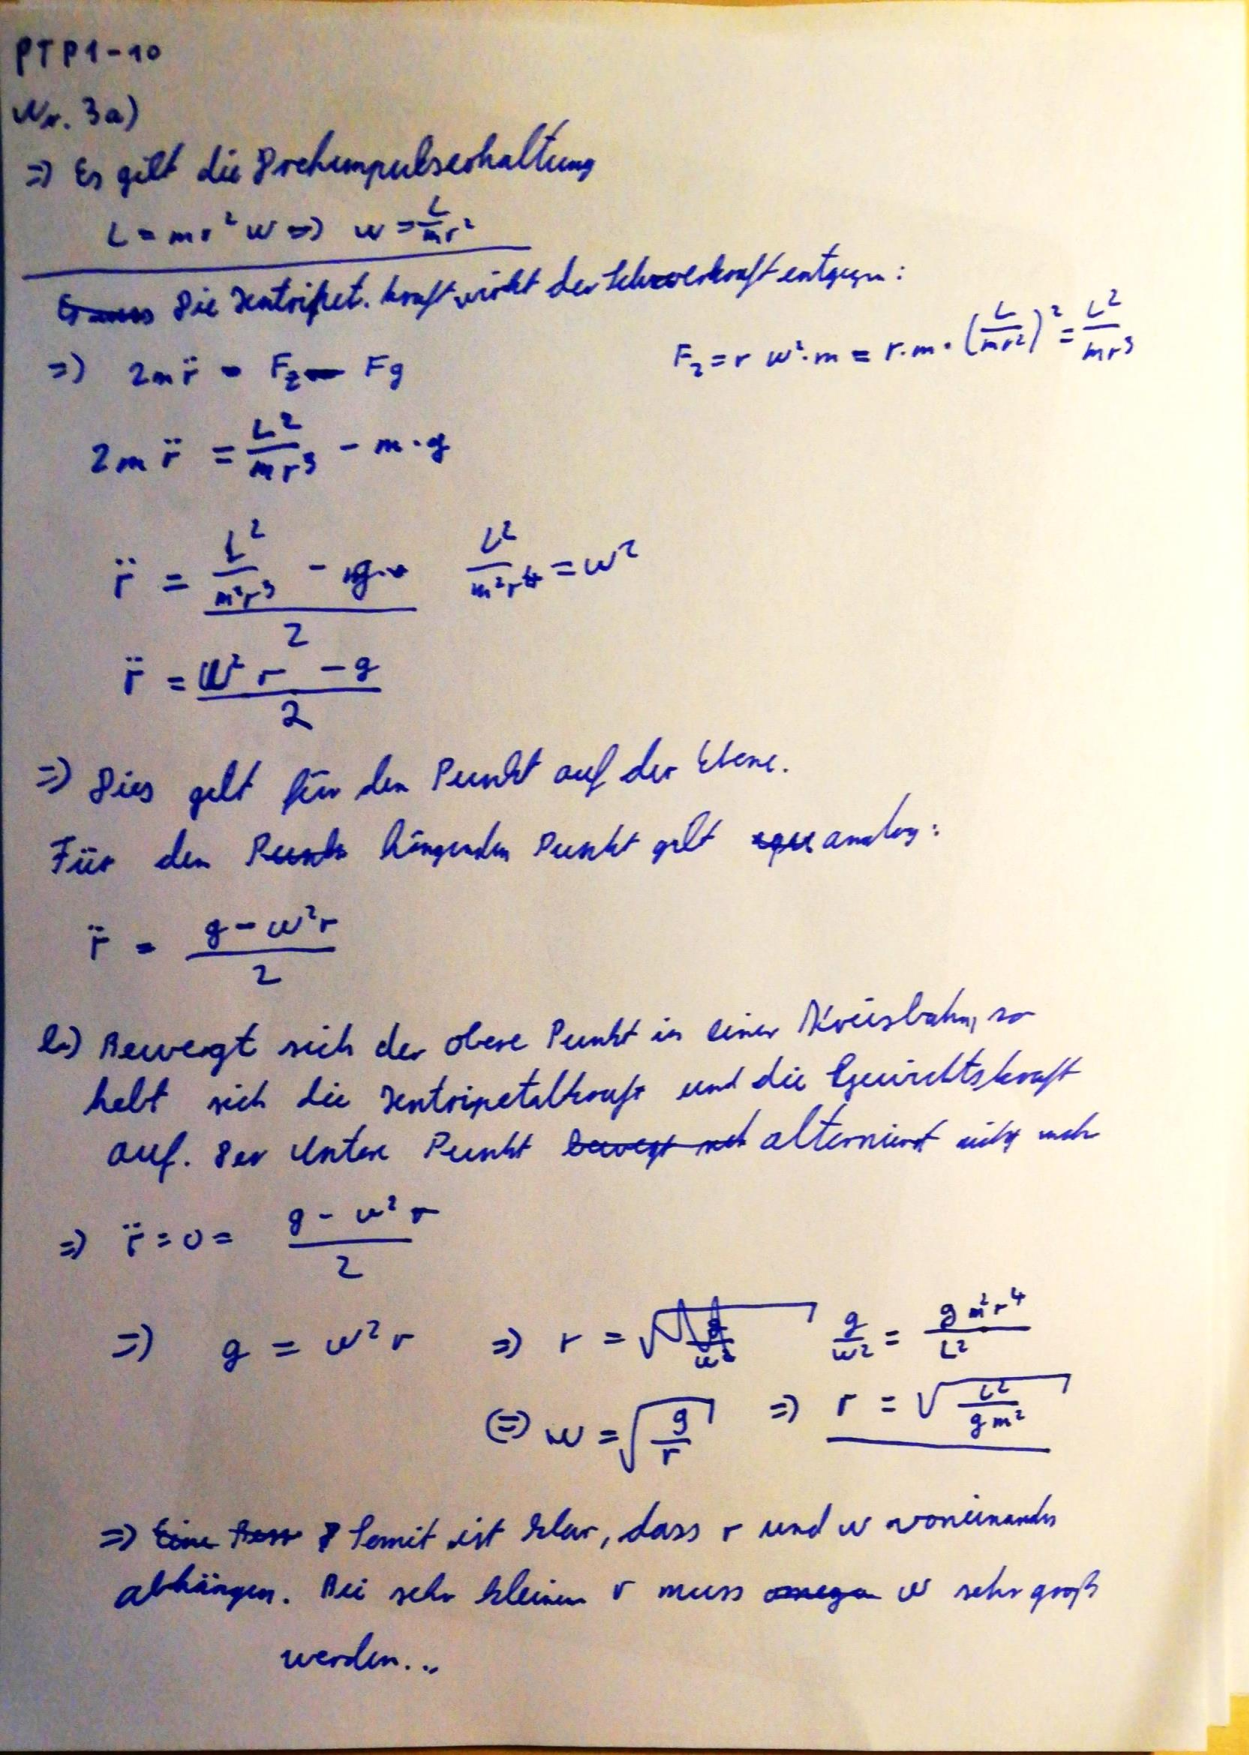
\includepdf[pages=-]{Theo1U10A3.pdf}


\section*{Aufgabe 10.4} 

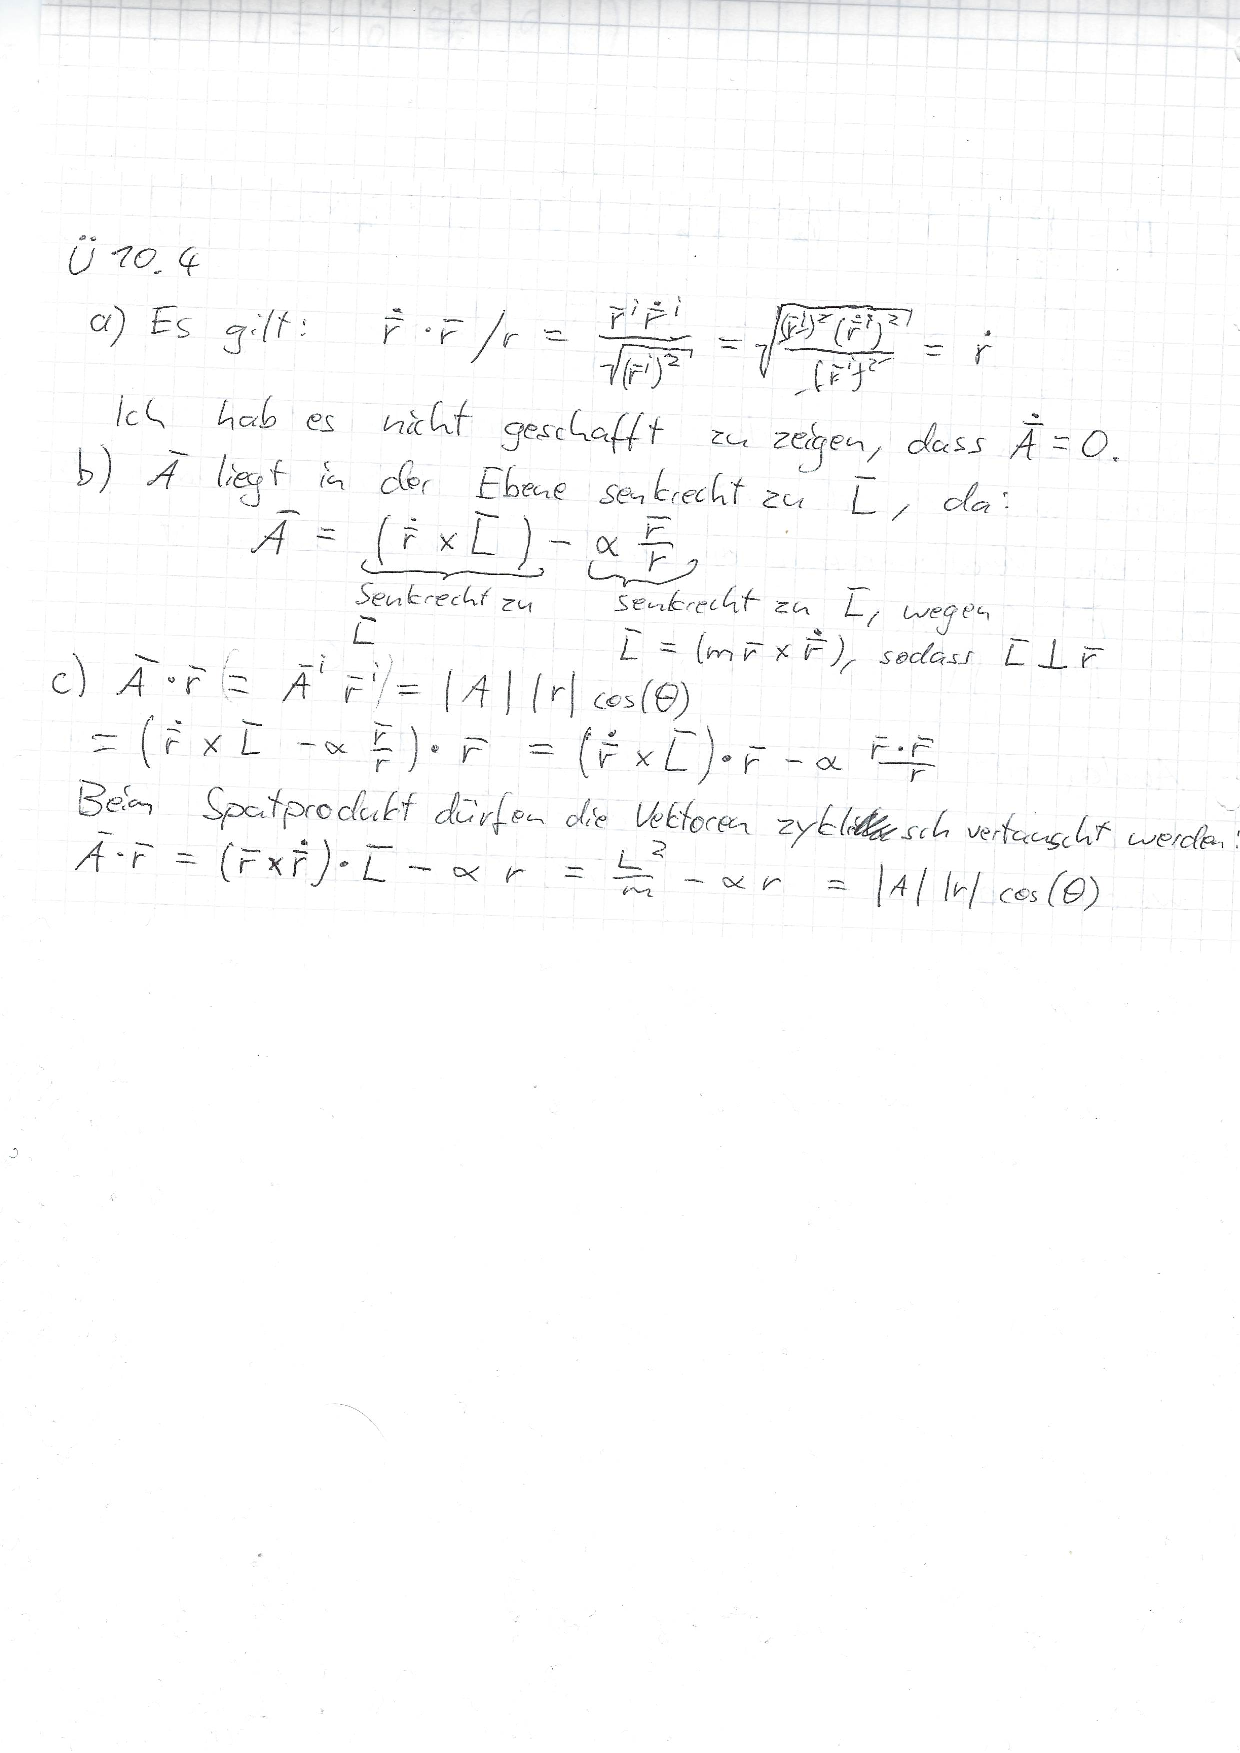
\includepdf[pages=-]{Theo1U10A4.pdf}


\section*{Aufgabe 10.5} 



\end{document}
